\documentclass[main.tex]{subfiles}

\begin{document}

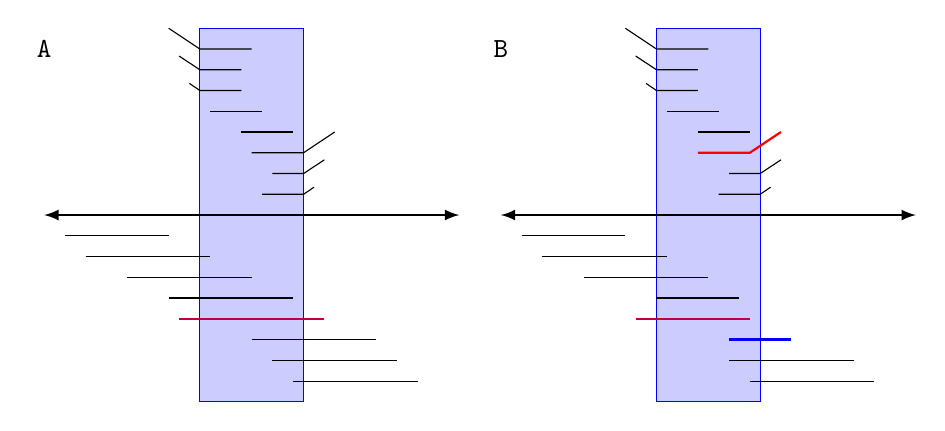
\begin{tikzpicture}[x=0.75pt,y=0.75pt,yscale=-1,xscale=1]

\draw [blue, fill=blue, fill opacity=0.2] (75, -90) -- (125, -90) -- (125, 90) -- (75, 90) -- cycle;

\draw (0, -80) node {\texttt{A}};
\draw (60, -90) -- (75, -80) -- (100, -80);
\draw (65, -76.6) -- (75, -70) -- (95, -70);
\draw (70, -63.4) -- (75, -60) -- (95, -60);
\draw (80, -50) -- (105, -50);
\draw (95, -40) -- (120, -40);
\draw (100, -30) -- (125, -30) -- (140, -40);
\draw (110, -20) -- (125, -20) -- (135, -26.6);
\draw (105, -10) -- (125, -10) -- (130, -13.4);
\draw  [fill opacity=1, <->, >=latex,thick,black] (0, 0) -- (200, 0);
\draw (10, 10) -- (60, 10);
\draw (20, 20) -- (80, 20);
\draw (40, 30) -- (100, 30);
\draw (60, 40) -- (120, 40);
\draw [fill opacity=1,thick,purple] (65, 50) -- (135, 50);
\draw (100, 60) -- (160, 60);
\draw (110, 70) -- (170, 70);
\draw (120, 80) -- (180, 80);

\draw [blue, fill=blue, fill opacity=0.2] (295, -90) -- (345, -90) -- (345, 90) -- (295, 90) -- cycle;

\draw (220, -80) node {\texttt{B}};
\draw (280, -90) -- (295, -80) -- (320, -80);
\draw (285, -76.6) -- (295, -70) -- (315, -70);
\draw (290, -63.4) -- (295, -60) -- (315, -60);
\draw (300, -50) -- (325, -50);
\draw (315, -40) -- (340, -40);
\draw [fill opacity=1,thick,red] (315, -30) -- (340, -30) -- (355, -40);
\draw (330, -20) -- (345, -20) -- (355, -26.6);
\draw (325, -10) -- (345, -10) -- (350, -13.4);
\draw  [fill opacity=1, <->, >=latex,thick,black] (220, 0) -- (420, 0);
\draw (230, 10) -- (280, 10);
\draw (240, 20) -- (300, 20);
\draw (260, 30) -- (320, 30);
\draw (295, 40) -- (335, 40);
\draw [fill opacity=1,thick,purple] (285, 50) -- (340, 50);
\draw [fill opacity=1,thick,blue] (330, 60) -- (360, 60);
\draw (330, 70) -- (390, 70);
\draw (340, 80) -- (400, 80);
\end{tikzpicture}

\end{document}